% Guides
% http://ivk.knteu.kiev.ua/docum/z_vg.pdf
% http://www.ivk.knteu.kiev.ua/docum/prav01.pdf
\documentclass[a4paper,14pt,oneside,final]{extarticle}
\usepackage[top=2cm, bottom=2cm, left=3cm, right=1cm]{geometry}
\usepackage{scrextend}

\usepackage[T2A,T1]{fontenc}
\usepackage[ukrainian,russian,english]{babel}
\usepackage{tempora}
\usepackage{fontspec}
\setmainfont{tempora}

% Зачем: Отключает использование изменяемых межсловных пробелов.
% Почему: Так не принято делать в текстах на русском языке.
\frenchspacing

\usepackage{indentfirst}
\setlength{\parindent}{1.25cm}
\renewcommand{\baselinestretch}{1.5}

% Header
\usepackage{fancyhdr}
\pagestyle{fancy}
\fancyhead{}
\fancyfoot{}
\fancyhead[R]{\small \selectfont \thepage}
\renewcommand{\headrulewidth}{0pt}

% Captions
\usepackage{chngcntr}
\counterwithin{figure}{section}
\counterwithin{table}{section}
\usepackage[tableposition=top]{caption}
\usepackage{subcaption}
\DeclareCaptionLabelFormat{gostfigure}{Рисунок #2}
\DeclareCaptionLabelFormat{gosttable}{Таблиця #2}
\DeclareCaptionLabelSeparator{gost}{~---~}
\captionsetup{labelsep=gost}
\captionsetup[figure]{labelformat=gostfigure}
\captionsetup[table]{labelformat=gosttable}
\renewcommand{\thesubfigure}{\asbuk{subfigure}}

% Sections
\usepackage[explicit]{titlesec}
\newcommand{\sectionbreak}{\clearpage}

\titleformat{\section}
  {\centering}{\thesection \quad}{0pt}{\MakeUppercase{#1}}
\titleformat{\subsection}[block]
  {\bfseries}{\thesubsection \quad #1}{0cm}{}

\titlespacing{\section} {0cm}{0cm}{21pt}
\titlespacing{\subsection} {\parindent}{21pt}{0cm}
\titlespacing{\subsubsection} {\parindent}{0cm}{0cm}

% Lists
\usepackage{enumitem}
\renewcommand\labelitemi{--}
\setlist[itemize]{noitemsep, topsep=0pt, wide}
\setlist[enumerate]{noitemsep, topsep=0pt, wide, label=\arabic*}
\setlist[description]{labelsep=0pt, noitemsep, topsep=0pt, leftmargin=2\parindent, labelindent=\parindent, labelwidth=\parindent, font=\normalfont}

% Toc
\usepackage{tocloft}
\tocloftpagestyle{fancy}
\renewcommand{\cfttoctitlefont}{}
\setlength{\cftbeforesecskip}{0pt}
\renewcommand{\cftsecfont}{}
\renewcommand{\cftsecpagefont}{}
\renewcommand{\cftsecleader}{\cftdotfill{\cftdotsep}}

\usepackage{float}
\usepackage{pgfplots}
\usepackage{graphicx}
\usepackage{multirow}
\usepackage{amssymb,amsfonts,amsmath,amsthm}
\usepackage{csquotes}

\usepackage{listings}
\lstset{basicstyle=\footnotesize\ttfamily,breaklines=true}
\lstset{language=Matlab}

\usepackage[
	backend=biber,
	sorting=none,
	language=auto,
	autolang=other
]{biblatex}
\DeclareFieldFormat{labelnumberwidth}{#1}

% Copied from
% https://github.com/cansik/kotlin-latex-listing
% big thanks to him!
\lstdefinelanguage{Kotlin}{
  keywords={package, as, as?, typealias, this, super, val, var, fun, for, null, true, false, is, in, throw, return, break, continue, object, if, try, else, while, do, when, class, interface, enum, object, companion, override, public, private, get, set, import, abstract, vararg, expect, actual, where, suspend, data, internal, dynamic, final, by},
  keywordstyle=\color{NavyBlue}\bfseries,
  ndkeywords={@Deprecated, @JvmName, @JvmStatic, @JvmOverloads, @JvmField, @JvmSynthetic, Iterable, Int, Long, Integer, Short, Byte, Float, Double, String, Runnable, Array},
  ndkeywordstyle=\color{BurntOrange}\bfseries,
  emph={println, return@, forEach, map, mapNotNull, first, filter, firstOrNull, lazy, delegate},
  emphstyle={\color{OrangeRed}},
  identifierstyle=\color{black},
  sensitive=true,
  commentstyle=\color{gray}\ttfamily,
  comment=[l]{//},
  morecomment=[s]{/*}{*/},
  stringstyle=\color{ForestGreen}\ttfamily,
  morestring=[b]",
  morestring=[s]{"""*}{*"""},
}


\usepackage{lastpage}
\usepackage{calc}
\usepackage{pdfpages}
\usepackage{soul}
\usepackage{pbox}
\usepackage{ulem}
\usepackage{titling}
\usepackage{framed}
\usepackage{tabu}
\usepackage{appendix}
\usepackage{packages/tikz-uml}
\usepackage[nomain,acronym,toc,nogroupskip,sort=def,xindy={glsnumbers=false}]{glossaries}
\usepackage[figure,table]{totalcount}

\makeglossaries
\newglossarystyle{mylist}{%  
 % put the glossary in the itemize environment:  
 \renewenvironment{theglossary}%  
   {\begin{itemize}[label={}]}{\end{itemize}}%  
 % have nothing after \begin{theglossary}:  
 \renewcommand*{\glossaryheader}{}%  
 % have nothing between glossary groups:  
 \renewcommand*{\glsgroupheading}[1]{}%  
 \renewcommand*{\glsgroupskip}{}%  
 % set how each entry should appear:  
 \renewcommand*{\glossentry}[2]{%  
 \item % bullet point  
 \glstarget{##1}{\glossentryname{##1}}% the entry name  
 \space ---% the symbol in brackets  
 \space \glossentrydesc{##1}% the description  
 %\space [##2]% the number list in square brackets
 .  
 }%  
 % set how sub-entries appear:  
 \renewcommand*{\subglossentry}[3]{%  
   \glossentry{##2}{##3}}%  
 } 
\setglossarystyle{mylist}
 
\lstset{language=Kotlin}
\graphicspath{{figures/}}

\setlength{\abovedisplayskip}{20pt}
\setlength{\belowdisplayskip}{20pt}

\addbibresource{bibliography.bib}

%http://tex.stackexchange.com/a/141831/79756
%There is a way to automatically map the language field to the langid field. The following lines in the preamble should be enough to do that.
%This command will copy the language field into the langid field and will then delete the contents of the language field. The language field will only be deleted if it was successfully copied into the langid field.
\DeclareSourcemap{ %модификация bib файла перед тем, как им займётся biblatex
    \maps{
        \map{% перекидываем значения полей language в поля langid, которыми пользуется biblatex
            \step[fieldsource=language, fieldset=langid, origfieldval, final]
            \step[fieldset=language, null]
        }
        \map[overwrite]{% перекидываем значения полей shortjournal, если они есть, в поля journal, которыми пользуется biblatex
            \step[fieldsource=shortjournal, final]
            \step[fieldset=journal, origfieldval]
        }
        \map[overwrite]{% перекидываем значения полей shortbooktitle, если они есть, в поля booktitle, которыми пользуется biblatex
            \step[fieldsource=shortbooktitle, final]
            \step[fieldset=booktitle, origfieldval]
        }
        \map[overwrite, refsection=0]{% стираем значения всех полей addendum
            \perdatasource{bibliography.bib}
            \step[fieldsource=addendum, final]
            \step[fieldset=addendum, null] %чтобы избавиться от информации об объёме авторских статей, в отличие от автореферата
        }
        \map[overwrite]{% перекидываем refbase в addendum, чтобы указать тип публикации (ВАК, Scopus, WoS) в конце ссылки
            \perdatasource{bibliography.bib}
            \step[fieldsource=refbase, final]
            \step[fieldset=addendum, origfieldval]
        }
        \map{% перекидываем значения полей numpages в поля pagetotal, которыми пользуется biblatex
            \step[fieldsource=numpages, fieldset=pagetotal, origfieldval, final]
            \step[fieldset=pagestotal, null]
        }
        \map{% если в поле medium написано "Электронный ресурс", то устанавливаем поле media, которым пользуется biblatex, в значение eresource.
            \step[fieldsource=medium,
            match=\regexp{Электронный\s+ресурс},
            final]
            \step[fieldset=media, fieldvalue=eresource]
        }
        \map[overwrite]{% стираем значения всех полей issn
            \step[fieldset=issn, null]
        }
        \map[overwrite]{% стираем значения всех полей abstract, поскольку ими не пользуемся, а там бывают "неприятные" латеху символы
            \step[fieldsource=abstract]
            \step[fieldset=abstract,null]
        }
        \map[overwrite]{ % переделка формата записи даты
            \step[fieldsource=urldate,
            match=\regexp{([0-9]{2})\.([0-9]{2})\.([0-9]{4})},
            replace={$3-$2-$1$4}, % $4 вставлен исключительно ради нормальной работы программ подсветки синтаксиса, которые некорректно обрабатывают $ в таких конструкциях
            final]
        }
        \map[overwrite]{ % добавляем ключевые слова, чтобы различать источники
            \perdatasource{bibliography.bib}
            \step[fieldset=keywords, fieldvalue={biblioexternal,bibliofull}]
        }
        \map[overwrite]{ % добавляем ключевые слова, чтобы различать источники
            \perdatasource{bibliography.bib}
            \step[fieldset=keywords, fieldvalue={biblioauthorvak,biblioauthor,bibliofull}]
        }
        \map[overwrite]{ % добавляем ключевые слова, чтобы различать источники
            \perdatasource{bibliography.bib}
            \step[fieldset=keywords, fieldvalue={biblioauthorscopus,biblioauthor,bibliofull}]
        }
        \map[overwrite]{ % добавляем ключевые слова, чтобы различать источники
        \perdatasource{bibliography.bib}
            \step[fieldset=keywords, fieldvalue={biblioauthorwos,biblioauthor,bibliofull}]
        }
        \map[overwrite]{ % добавляем ключевые слова, чтобы различать источники
        \perdatasource{biblio/authorwos.bib}
            \step[fieldset=keywords, fieldvalue={biblioauthorother,biblioauthor,bibliofull}]
        }
        \map[overwrite]{ % добавляем ключевые слова, чтобы различать источники
        \perdatasource{biblio/authorother.bib}
            \step[fieldset=keywords, fieldvalue={biblioauthorconf,biblioauthor,bibliofull}]
        }
%        \map[overwrite]{% стираем значения всех полей series
%            \step[fieldset=series, null]
%        }
        \map[overwrite]{% перекидываем значения полей howpublished в поля organization для типа online
            \step[typesource=online, typetarget=online, final]
            \step[fieldsource=howpublished, fieldset=organization, origfieldval]
            \step[fieldset=howpublished, null]
        }
        % Так отключаем [Электронный ресурс]
%        \map[overwrite]{% стираем значения всех полей media=eresource
%            \step[fieldsource=media,
%            match={eresource},
%            final]
%            \step[fieldset=media, null]
%        }
    }
}

%%% Тире как разделитель в библиографии традиционной руской длины:
\renewcommand*{\newblockpunct}{\addperiod\addnbspace\cyrdash\space\bibsentence}

%%% В списке литературы обозначение одной буквой диапазона страниц англоязычного источника %%%
\DefineBibliographyStrings{english}{%
    pages = {p\adddot} %заглавность буквы затем по месту определяется работой самого biblatex
}

%%% Исправление длины тире в диапазонах %%%
% \cyrdash --- тире «русской» длины, \textendash --- en-dash
\DefineBibliographyExtras{russian}{%
  \protected\def\bibrangedash{%
    \cyrdash\penalty\value{abbrvpenalty}}% almost unbreakable dash
  \protected\def\bibdaterangesep{\bibrangedash}%тире для дат
}
\DefineBibliographyExtras{english}{%
  \protected\def\bibrangedash{%
    \cyrdash\penalty\value{abbrvpenalty}}% almost unbreakable dash
  \protected\def\bibdaterangesep{\bibrangedash}%тире для дат
}


\colorlet{punct}{red!60!black}
\definecolor{delim}{RGB}{20,105,176}
\colorlet{numb}{magenta!60!black}

\lstdefinelanguage{json}{
    basicstyle=\normalfont\ttfamily,
    numbers=left,
    numberstyle=\scriptsize,
    stepnumber=1,
    numbersep=8pt,
    showstringspaces=false,
    breaklines=true,
    literate=
     *{0}{{{\color{numb}0}}}{1}
      {1}{{{\color{numb}1}}}{1}
      {2}{{{\color{numb}2}}}{1}
      {3}{{{\color{numb}3}}}{1}
      {4}{{{\color{numb}4}}}{1}
      {5}{{{\color{numb}5}}}{1}
      {6}{{{\color{numb}6}}}{1}
      {7}{{{\color{numb}7}}}{1}
      {8}{{{\color{numb}8}}}{1}
      {9}{{{\color{numb}9}}}{1}
      {:}{{{\color{punct}{:}}}}{1}
      {,}{{{\color{punct}{,}}}}{1}
      {\{}{{{\color{delim}{\{}}}}{1}
      {\}}{{{\color{delim}{\}}}}}{1}
      {[}{{{\color{delim}{[}}}}{1}
      {]}{{{\color{delim}{]}}}}{1},
}


\setcounter{secnumdepth}{4}
\setcounter{tocdepth}{4} 

\titleformat{\paragraph}[block]
  {\bfseries}{\hspace*{1.25cm}\theparagraph \quad #1}{0cm}{}
\titleformat{name=\paragraph,numberless}[block]
  {\bfseries}{\hspace*{1.25cm}#1}{0cm}{}

\titlespacing{\paragraph} {0cm}{0cm}{0cm}

\newacronym{am}{АМ}{агентне моделювання}
\newacronym{gis}{ГІС}{геоінформаційна система}
\newacronym{computer}{ЕОМ}{електронна обчислювальна машина}
\newacronym{mas}{МАС}{мультиагентна система}
\newacronym{pc}{ПЕОМ}{персональна електронна обчислювальна машина}
\newacronym{sw}{ПЗ}{програмне забезпечення}
\newacronym{smw}{СУОП}{система управління охороною праці}

%\newacronym{afapl}{AFAPL}{Agent Factory Agent Programming Language}
%\newacronym{api}{API}{Application Programming Interface}
%\newacronym{corba}{CORBA}{Common Object Request Broker Architecture}
%\newacronym{fipa}{FIPA}{Foundation for Intelligent Physical Agents}
%\newacronym{faq}{FAQ}{Frequently Asked Questions}
%\newacronym{lgpl}{LGPL}{GNU Lesser General Public License}
%\newacronym{gui}{GUI}{Graphical User Interface}
%\newacronym{jade}{JADE}{Java Agent Development Framework}
%\newacronym{jre}{JRE}{Java Runtime Environment}
%\newacronym{jvm}{JVM}{Java Virtual Machine}
%\newacronym{json}{JSON}{JavaScript Object Notation}
%\newacronym{uml}{UML}{Unified Modeling Language}

\newcommand{\khpistudentgroup}{КН-34г}
\newcommand{\khpistudentname}{Чепурний~А.~С.}

\newcommand{\khpidepartment}{Програмна інженерія та інформаційні технології управління}
\newcommand{\khpititlewhat}{
	Лабораторна робота №\labnumber \\
	з предмету <<Моделювання систем>>
}
\newcommand{\khpititlewho}{
	Виконав: \\
	\hspace*{\parindent} ст. групи \khpistudentgroup \\
	\hspace*{\parindent} \khpistudentname \\
	Перевірила: \\
	\hspace*{\parindent} ст. в. каф. ПІІТУ \\
	\hspace*{\parindent} Єршова~С.~І. \\
	\hspace*{\parindent} ас. каф. ПІІТУ \\
	\hspace*{\parindent} Литвинова~Ю.~С. \\
}


\begin{document}
\Ukrainian

\begin{titlepage}
\includepdf[pages=-]{title/DOC_PRAK_6k_mag_n}
\end{titlepage}

\addtocounter{page}{1}
\renewcommand\contentsname{\hspace*{\fill}\bfseries\MakeUppercase{Зміст}\hspace*{\fill}}
\tableofcontents

\printglossary[type=\acronymtype,title={Перелік позначень та скорочень}]


\section*{Вступ}
\addcontentsline{toc}{section}{Вступ}
На сучасному етапі розвитку складні логістичні системи вимушені працювати в умовах високої невизначеності, що суттєво ускладнює управління ними. 
В процесі прийняття управлінських рішень виникає проблема прогнозування поведінки системи та зовнішнього середовища. 
Результати прогнозів необхідно постійно коригувати по ходу розвитку подій, що дозволяє пристосовуватися до змін оточення та гнучко реагувати на негативні впливи. 

У нагоді тут стає агентне моделювання, яке сягає своїм історичним корінням складних адаптивних систем і принципу побудови систем знизу вгору.
Агентне моделювання дозволяє здійснити множину прогнозів за різними сценаріями залежно від формування різноманітних ситуацій практично необмеженої складності. 

Основними елементами агентного моделювання є агенти, стосунки між ними і простір, в якому відбувається взаємодія. 
Агенти моделюються індивідуально. 
Вони можуть мати неповну інформацію, здійснювати помилки, адаптуватися до ситуації, проявляти ініціативу. 
В основу агентного моделювання закладені такі принципи, як різноманітність, взаємозв’язок і міра взаємодії. 
Тип взаємодій різних агентів може відрізнятися і носити ймовірнісний характер. 
Результатом динамічної взаємодії може бути певний рівноважний стан системи, а може бути і нова якість, яку неможливо передбачати з аналізу окремих складових системи.

Об'єктом дослідження є процес агентного моделювання логістичної системи. 

Предметом дослідження є моделі та інструментальні засоби розробки системи для оцінки рівня сервісу логістичних систем дистрибуції.

Теоретико-методологічною основою роботи є агентне моделювання, системний аналіз, а також базова теорія логістики.

Метою дослідження є розробка та дослідження моделей та програмна реалізація інформаційної системи для визначення рівня сервісу логістичної системи.
Для досягнення поставленої мети в дипломній роботі були сформульовані та вирішені наступні задачі:
\begin{itemize}
	\item описати вимоги до програмної системи;
	\item на основі аналізу вимог запропонувати варіант цільової архітектури;
	\item на основі результатів аналізу затвердити кінцевий варіант цільової архітектури для реалізації у програмній компоненті моделювання мережевого сервісу логістичної системи дистрибуції;
	\item розробити програмну компоненту на базі прийнятого архітектурного рішення;
	\item провести тестування розробленої програмної системи;
	\item провести експеримент та проаналізувати його результати.
\end{itemize}

\section{Результати застосування розробленої системи}
\subsection{Стислі відомості щодо розгортання системи}

Вимоги до серверної машини наведено у таблиці~\ref{tab:sw_requirements}. 

\begin{table}[h]
	\caption{Мінімальні вимоги до серверного обладнання}
	\label{tab:sw_requirements}
	\begin{tabular}{l|l}
		Процесор & 1000 МГц \\ \hline
		ОЗП & 512 МБ \\ \hline
		Об'єм пам'яті диску & 64 ГБ 
	\end{tabular}
\end{table}

Програмне забезпечення серверу може бути встановлено на операційні системи родини \textit{Linux}, \textit{Windows} або \textit{macOS}.
Рекомендовано використовувати \acrshort{ssd} у якості накопичувача.

Для розгортання системи необхідно встановити наступні програми:
\begin{itemize}
	\item Apache Server v2.4.29+;
	\item SQLite v3.22.0+;
	\item PHP v7.2.2+;
\end{itemize}
та встановити драйвер взаємодії PHP з SQLite.

\subsection{Опис роботи з сайтом}
Робота з сайтом починається з процесу реєстрації користувача~(рисунок~\ref{fig:site_register}).
Незареєстрований користувач може переглядати товари та додавати їх до кошику, але не може оформити замовлення. 
\begin{figure}[H]
    \centering
    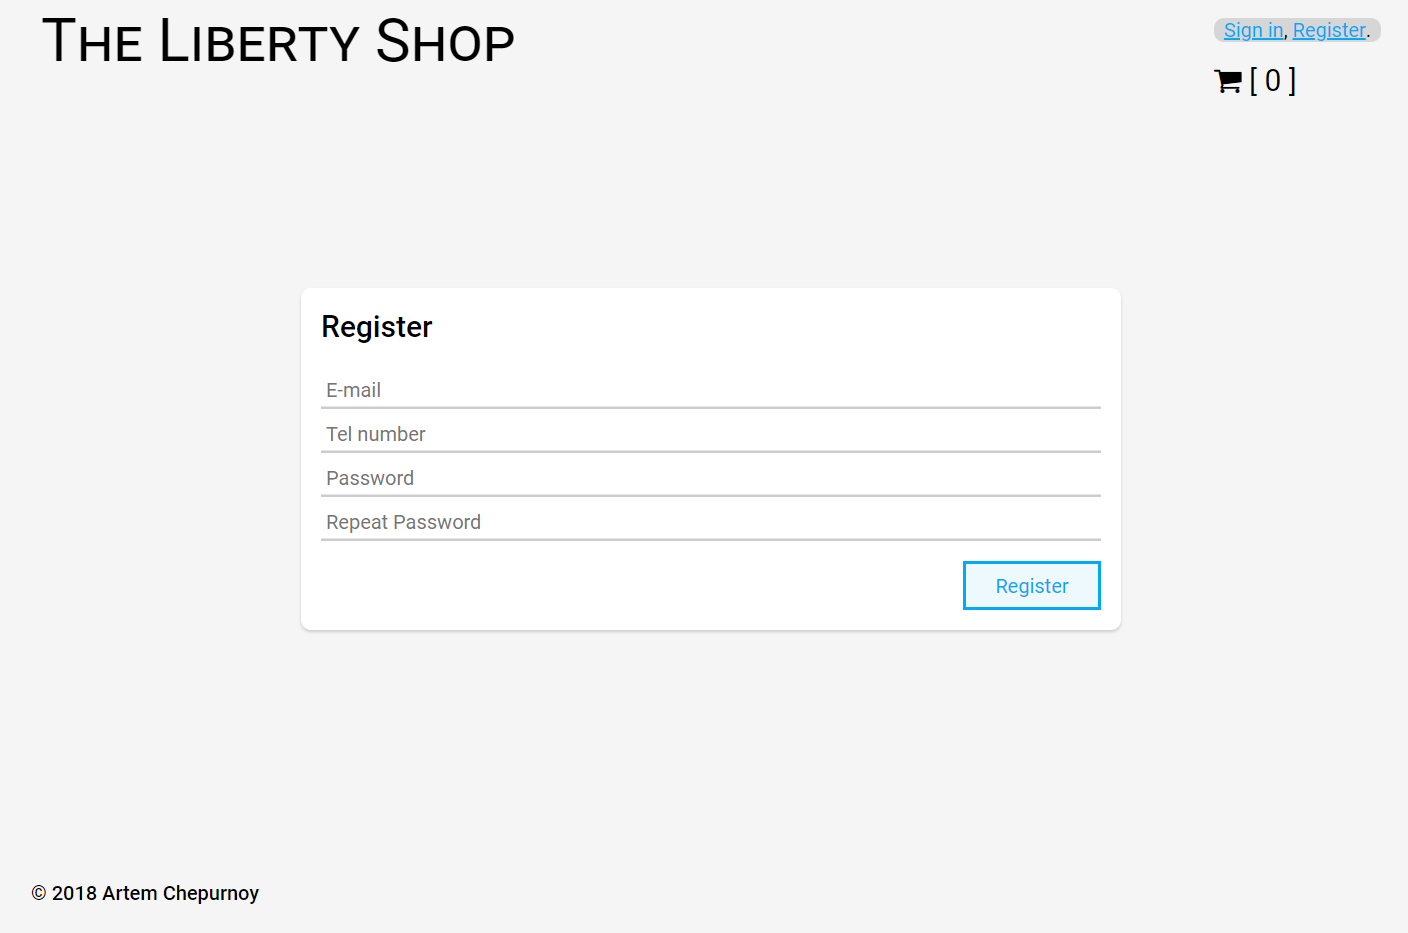
\includegraphics[width=0.8\textwidth]{screen_register}
    \caption{Сторінка реєстрації у системі}
    \label{fig:site_register}
\end{figure}

Після реєстрації користувач має увійти до системи~(рисунок~\ref{fig:site_login}).
\begin{figure}[H]
    \centering
    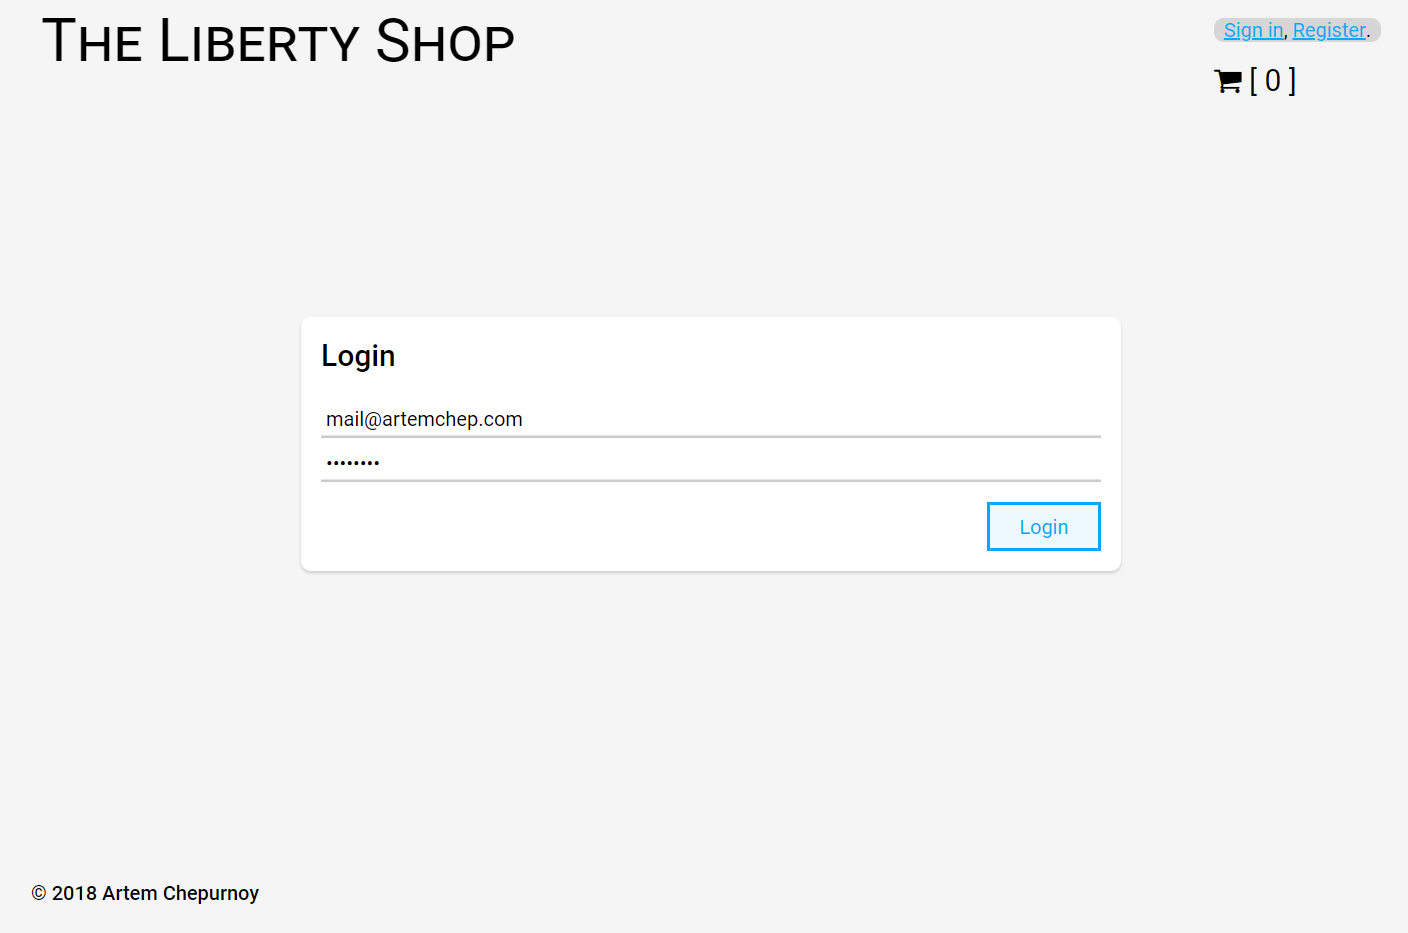
\includegraphics[width=0.8\textwidth]{screen_login}
    \caption{Сторінка входу до системи}
    \label{fig:site_login}
\end{figure}

Користувач може переглядати доступні товари на головній сторінці сайту.
Доступна можливість пошуку товару за ім'ям та категоріям.
\begin{figure}[H]
    \centering
    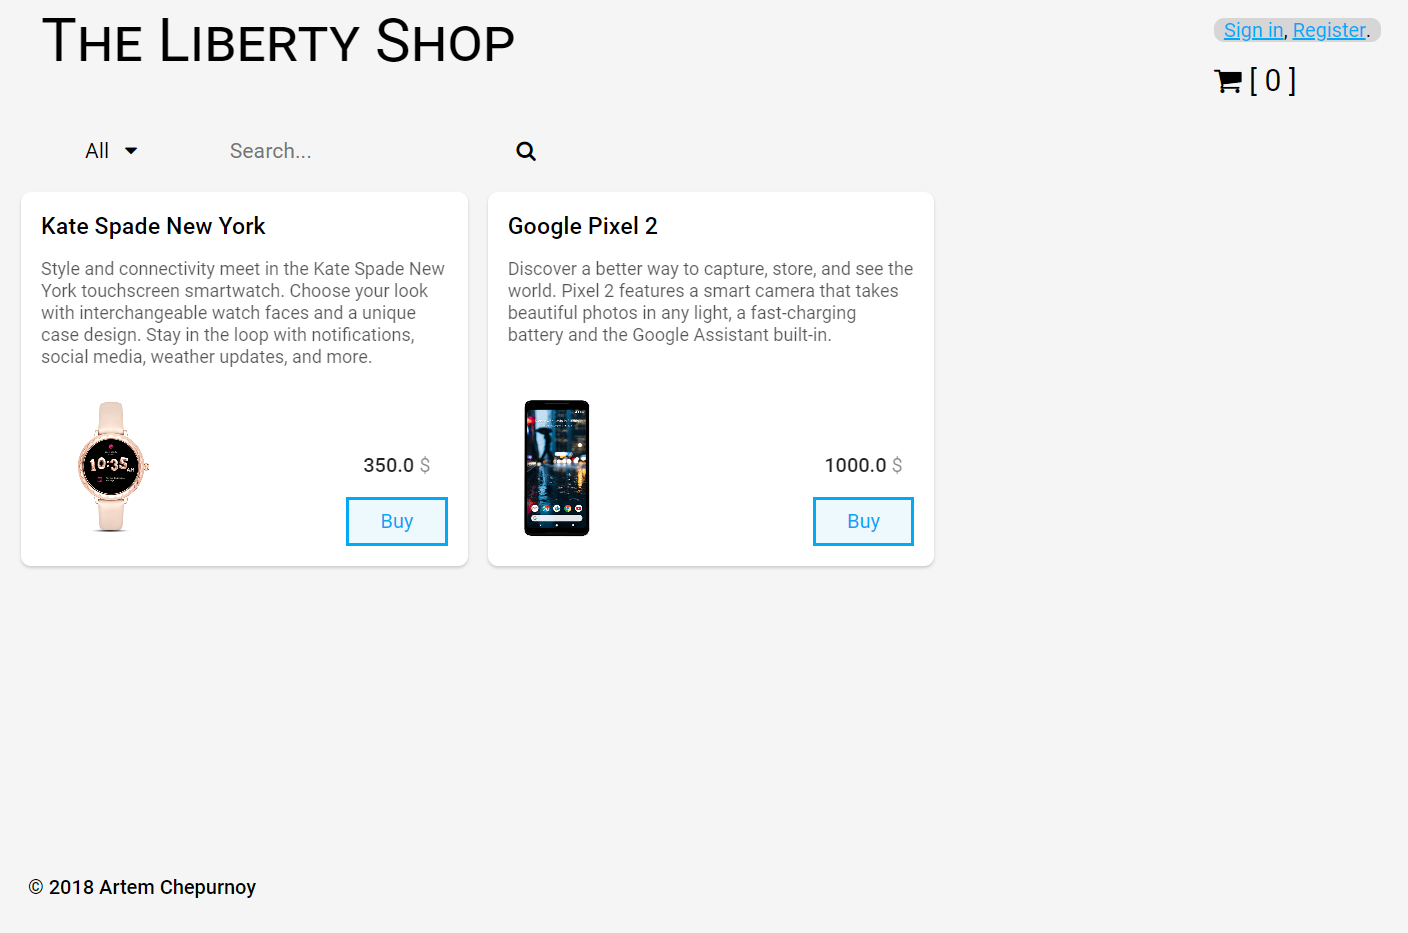
\includegraphics[width=0.8\textwidth]{screen_product__list}
    \caption{Головна сторінка ресурсу}
    \label{fig:site_product_list}
\end{figure}

Адміністратор та менеджери сайту мають на головній сторінці додаткові елементи~(рисунок~\ref{fig:site_product_list_admin}): 
\begin{itemize}
\item Кнопка редагування продуктів;
\item \textit{<<Add product>>} --- показати діалог додавання нового продукту;
\item \textit{<<Add category>>} --- показати діалог додавання нової категорії продуктів;
\item \textit{<<Edit category>>} --- показати діалог редагування та видалення категорії продуктів.
\end{itemize}
\begin{figure}[H]
    \centering
    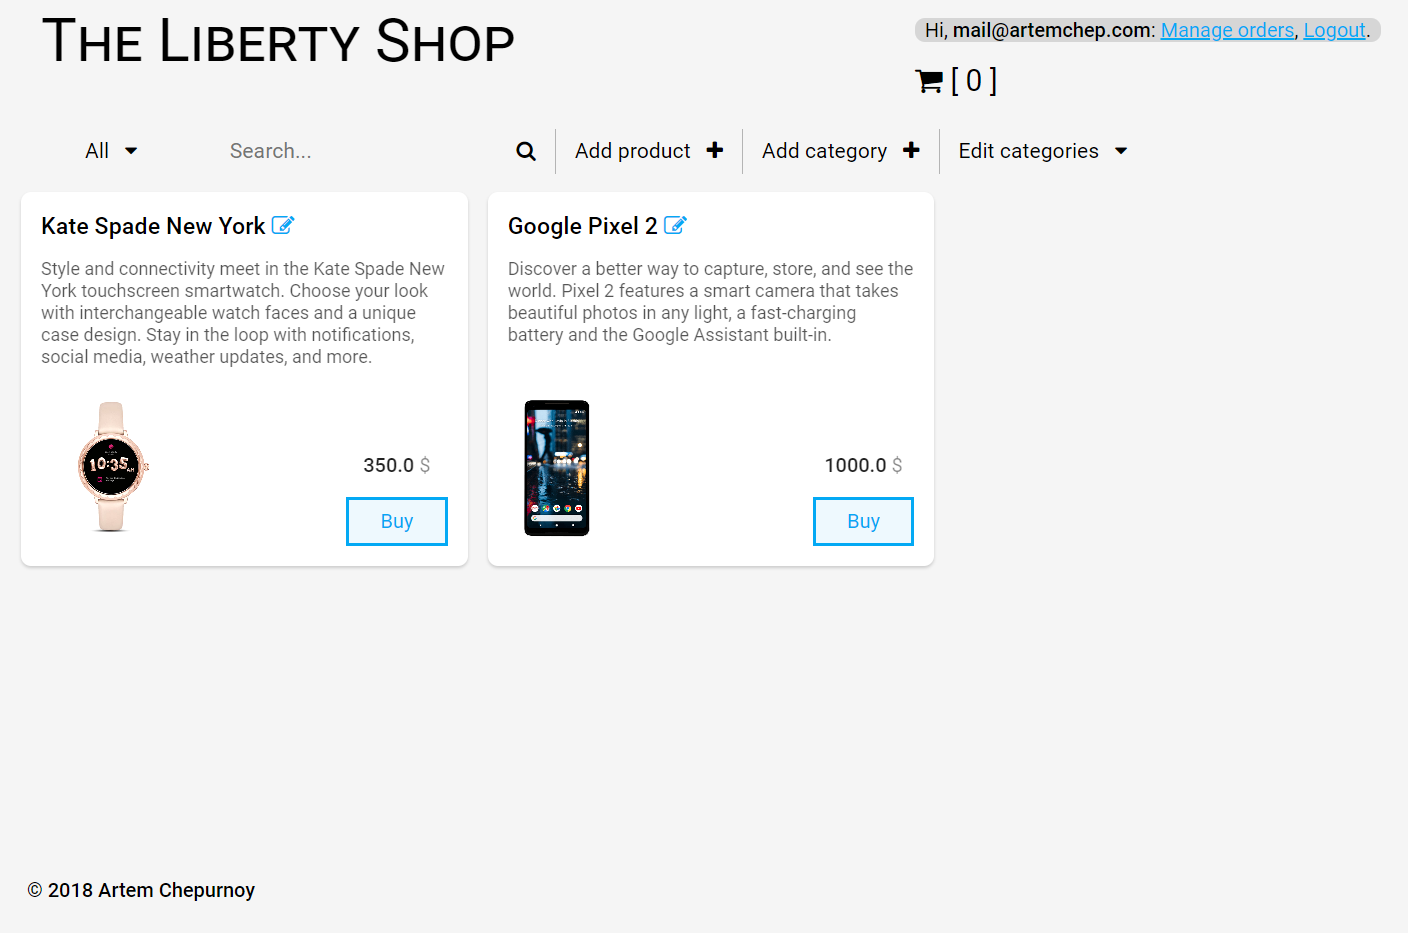
\includegraphics[width=0.8\textwidth]{screen_product__list__admin}
    \caption{Головна сторінка ресурсу (адміністратор)}
    \label{fig:site_product_list_admin}
\end{figure}

Діалог для створення нового продукту представлено на рисунку~\ref{fig:site_product_add}).

Продукт має такі властивості як категорія продуктів, назва, короткий опис, графічне зображення, ціна та розмірність.   
\begin{figure}[H]
    \centering
    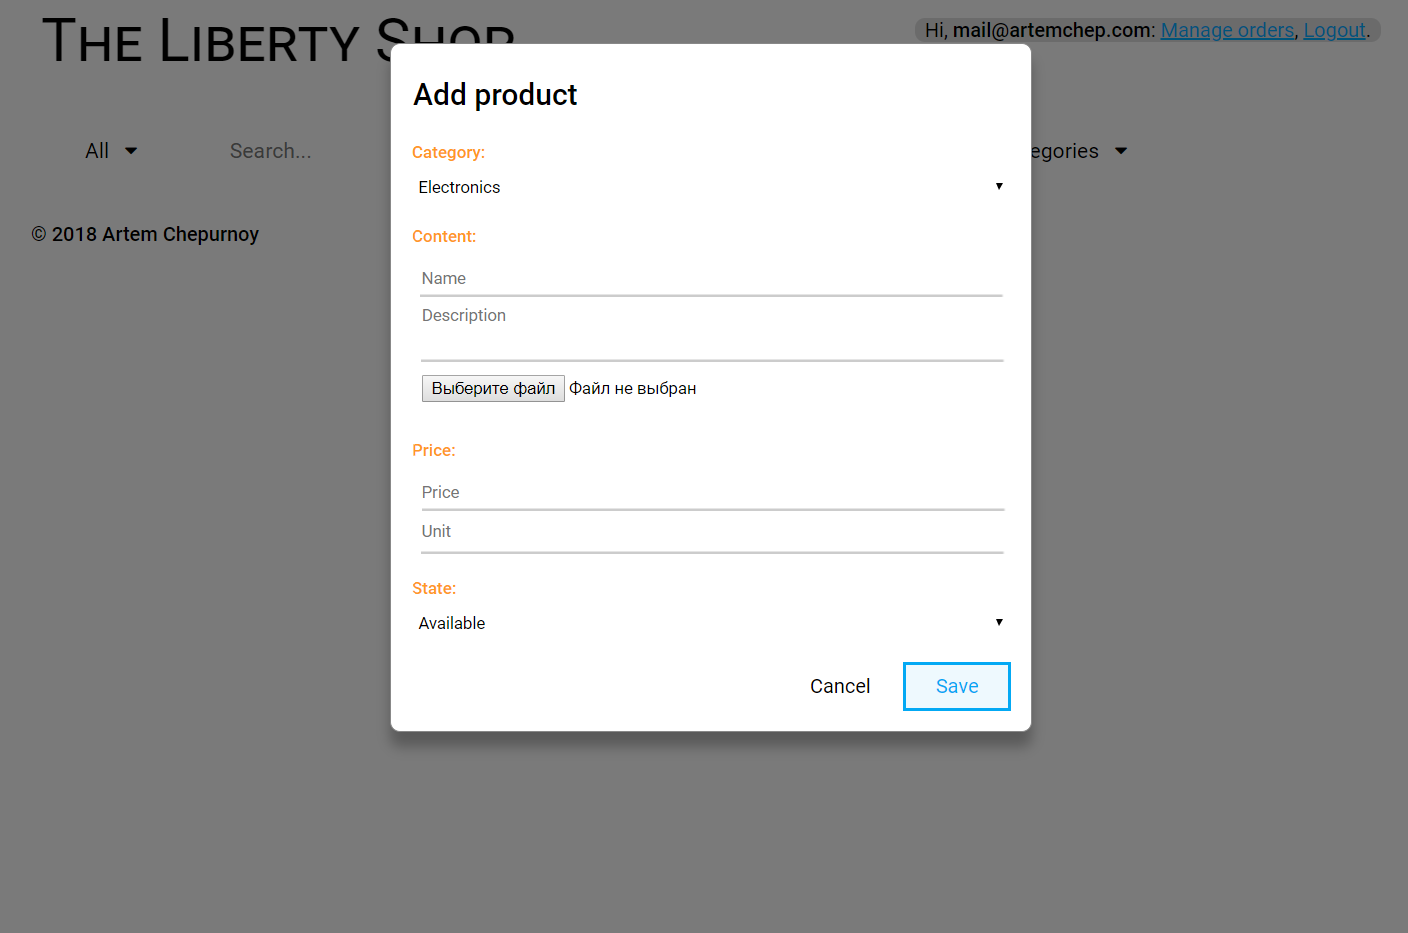
\includegraphics[width=0.8\textwidth]{screen_product_add}
    \caption{Діалог створення нового продукту}
    \label{fig:site_product_add}
\end{figure}

Адміністратор та менеджер ресурсу мають можливість переглянути список поточних або минулих замовлень~(рисунок~\ref{fig:site_order_list}), перемістити замовлення до архіву.
Є можливість фільтрування замовлень по даті створення, даті архівування, назві, категорії, кількості продуктів та ціні.   
\begin{figure}[H]
    \centering
    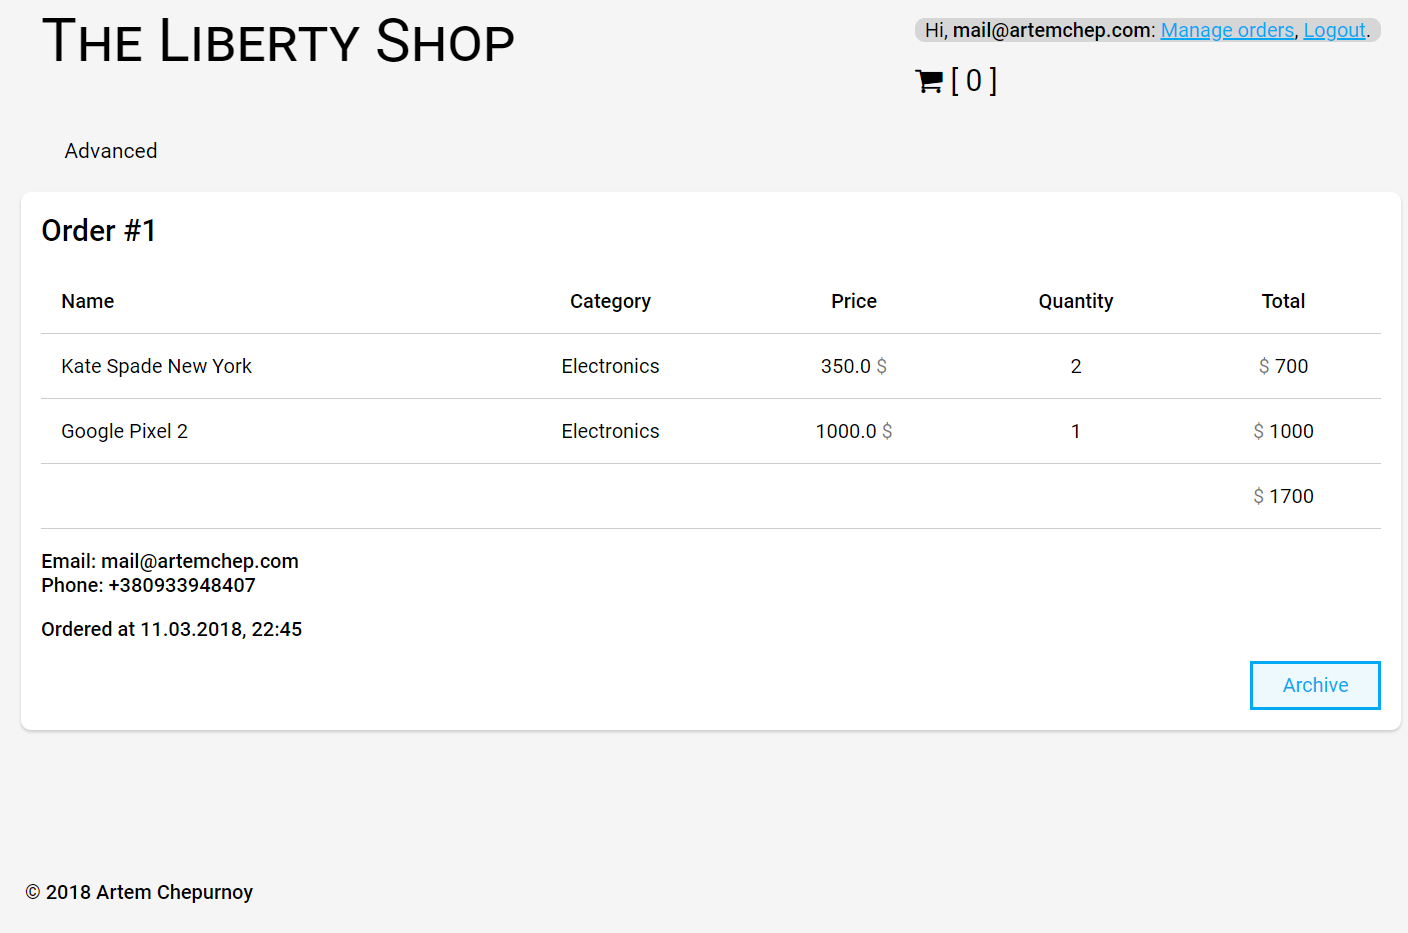
\includegraphics[width=0.8\textwidth]{screen_order__list}
    \caption{Сторінка керування замовленнями}
    \label{fig:site_order_list}
\end{figure}

\subsection{Результати тестування та рекомендації щодо удосконалення розробленої системи}
При тестуванні основною проблемою виявилася підтримка сайтом різних пристроїв та браузерів. 
При більш детальному вивченні стандартів HTML та CSS ця проблема була вирішена.

Одним із напрямків розвитку розробленої системи є співробітництво з іншими постачальниками, створення платформи для постачальників. 

\section{Програмна реалізація системи}
\subsection{Особливості програмної реалізації системи, що розробляється}
Для розробки програмної системи була використані мова програмування Kotlin та застосовані патерни проектування типу GoF.

Були застосовані принципи SOLID~\cite{Arch2007}:
\begin{enumerate}
	\item Принцип єдиного обов'язку --- принцип об'єктно-орієнтованого програмування, який означає, що клас має бути створений для виконання лише однієї задачі, яку він повинен повністю інкапсулювати.
	      Отже, всі сервіси цього класу мають бути повністю підпорядковані її виконанню.
	      Результатом слідування цій концепції є наявність лише однієї причини для зміни класу.
	\item Принцип відкритості/закритості --- принцип об'єктно-орієнтованого програмування, який означає, що програмні сутності, такі як класи, модулі, функції, методи та ін. мають бути <<відкритими для розширення та закритими для змін>>.
	      Це означає, що вони можуть надавати можливість змінювати свою поведінку без або з мінімальними змінами коду.
	\item Принцип заміщення Лісков --- якщо $S$ підтип $T$, тоді об'єкти типу $T$ в програмі можуть бути заміщені об'єктами типу $S$ без будь-яких змін бажаних властивостей цієї програми.
	\item Принцип розділення інтерфейсів --- принцип схожий із принципом єдиного обов'язку.
	      Застосування даного принципу полягає у розділі занадто <<товстих>> інтерфейсів на менші та специфічні, щоб їх клієнти знали лише про ті методи, що необхідні для них у роботі.
	      Як результат, при зміні певного функціоналу, незмінними мають лишитися ті класи, що не використовують його.
	      Тобто виконання цього принципу допомагає системі залишатися гнучкою при внесенні до неї змін та лишатися простою для рефакторингу.
	\item Принцип інверсії залежностей.
	      Принцип формулюється наступним чином: модулі вищого рівня не повинні залежати від модулів нижчого рівня, обидва типи модулів повинні залежати від абстракцій; абстракції не повинні залежати від деталей реалізації, деталі реалізації повинні залежати від абстракцій.
\end{enumerate}

Система реалізована у парадігмі чистої архітектури, яка полягає в розділенні системи на 3 рівні~\cite{Arch2007}:
\begin{enumerate}
	\item Рівень даних --- рівень даних у чистому вигляді, що складається з сутностей, які є основними бізнес-правилами системи.
	\item Доменний рівень --- рівень бізнес-логіки додатку, що відповідає за основний функціонал системи, її поведінку та правила, що стосуються конкретного додатку.
	\item Рівень представлення --- рівень користувацького інтерфейсу, відображення даних, обробки користувацьких подій.
\end{enumerate}

\subsection{Тестування програмного забезпечення}
\subsubsection{Загальна теорія тестування}
Тестування --- перевірка відповідності реальної поведінки програми очікуваній, що здійснюється на кінцевому наборі тестів, який був обраний певним чином.
У більш широкому сенсі, тестування --- це одна з технік контролю якості, що включає в себе активності з планування робіт, проектування тестів, виконання тестування і аналізу отриманих результатів~\cite{Swebok}.

Верифікація --- це процес оцінки системи або її компонентів з метою визначення чи задовольняють результати поточного етапу розробки умовам, що були сформовані на початку цього етапу.
Тобто чи виконуються наші цілі, терміни, завдання по розробці проекту, визначені на початку поточної фази~\cite{Swebok}.

Валідація --- це визначення відповідності ПО, що розроблюється очікуванням і потребам користувача, вимогам до системи~\cite{Swebok}.

\subsubsection{Тестування програмної системи}
На першому етапі тестування необхідно провести модульне тестування усіх компонентів системи, які можуть бути протестовані окремо від інших у штучному середовищі тестування.
Для Unit-тестування використовується засоб автоматизації тестування Kotest.

Такий вибір зумовлений простотою інтеграції з Kotlin.
Kotest надає великий об'єм валідаційних методів, завдяки яким можна легко та ефективно тестувати як модулі обробки даних та взаємодії з базами даних, так і модулі вводу та виводу інформації~\cite{Kotest}.

Фрагмент застосованих Kotest тестів для валідації коректної роботи класу \texttt{GlobeHipster} приведено нижче:
\lstinputlisting{code/tests.kt}

\subsection{Інтерфейс програмного забезпечення}
Розроблена програмна система має консольний інтерфейс. Для запуску моделювання необхідно виконати такі команди:
\begin{lstlisting}
> jar kagent.jar --period=14 --time=5 configuration_a.json configuration_b.json
\end{lstlisting}
\begin{description}
	\item[де] \texttt{kagent.jar} --- назва бінарного файла програмної системи;
	\item \texttt{--period=14} --- період поповнення запасів регіональними та національними складами, у днях;
	\item \texttt{--time=5} --- час моделювання системи, у секундах;
	\item \texttt{configuration\_a.json} --- шлях до файлу конфігурації першого варіанта логістичної системи;
	\item \texttt{configuration\_b.json} --- шлях до файлу конфігурації другого варіанта логістичної системи.
\end{description}

В процесі моделювання логістичної системи у консоль виводиться поточний стан логістичної системи.
Фрагмент логування початкової загрузки конфігурації логістичної системи:
\begin{lstlisting}
Connecting Киев to Пирятин by 154.0 km. road
Connecting Житомир to Винница by 127.0 km. road
Connecting Николаев to Мелитополь by 299.0 km. road
Connecting Николаев to Саки by 325.0 km. road
Connecting Днепропетровск to Днепродзержинск by 45.0 km. road
Connecting Львов to Дубляны by 9.0 km. road
\end{lstlisting}

Фрагмент логування процесу моделювання логістичної системи:
\begin{lstlisting}
[432]
.     Current time is 432 days.
.    service level is 87%.
. avg. stock level is 92%.
[433]
.     Current time is 433 days.
.    service level is 88%.
. avg. stock level is 92%.
[434]
.     Current time is 434 days.
.    service level is 88%.
. avg. stock level is 91%.
\end{lstlisting}

Для генерації дампу поточного стану системи у файл необхідно натиснути клавішу <<S>> під час процесу моделювання, для призупинення виконування програми необхідно натиснути клавішу <<P>>.
Графічний інтерфейс складається з двох частин: меню та панелі поточного стану моделі.

Після закінчення часу на моделювання системи показується окно з динамікою зміни рівня сервісу за час моделювання (рисунок~\ref{fig:graph_sample}).

\begin{figure}[H]
	\centering
	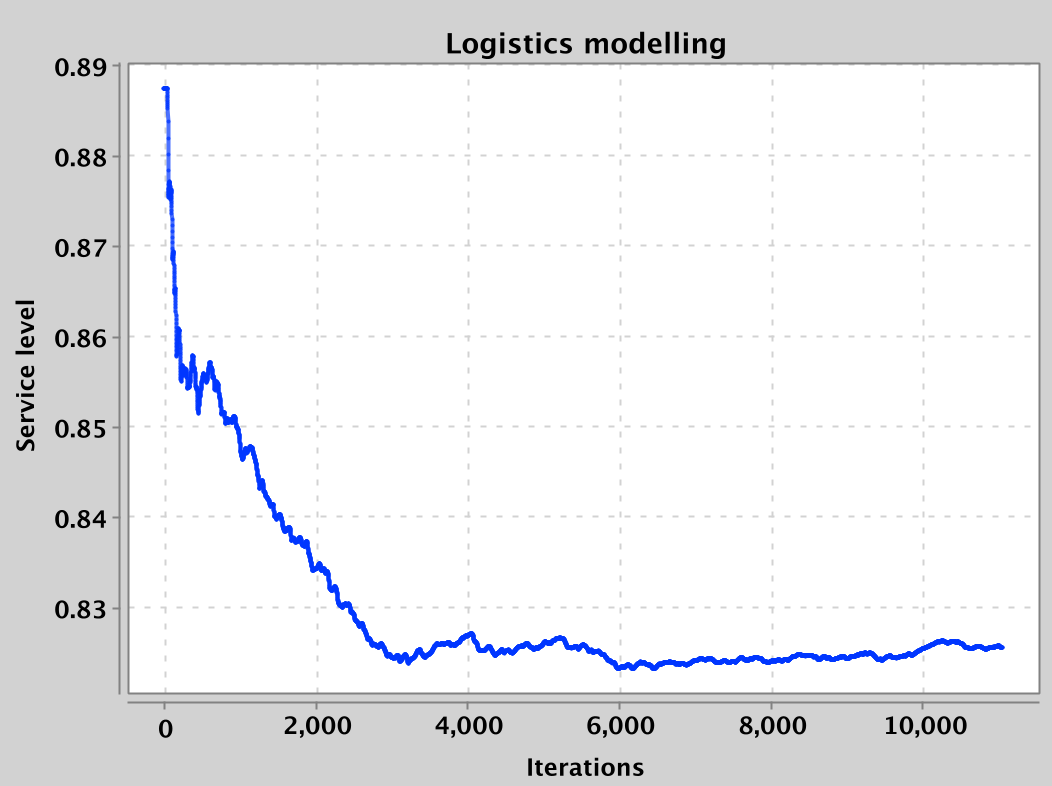
\includegraphics[width=0.6\textwidth]{graph_sample}
	\caption{Динаміка зміни рівня сервісу}
	\label{fig:graph_sample}
\end{figure}

\subsection{Аналіз продуктивності програмного забезпечення}
Розроблений програмний продукт широко використовує паралельні обчислення. 
В якості основи для паралельних обчислень було використано технологію Kotlin coroutines.

Для порівняння роботи програми у багатопотоковому режимі та однопотоковому режимі був проведений експеримент: моделювання логістичної системи~\cite{Годлевський2019} з обмеженої кількістю агентів на регіональному шару. Результат експерименту представлено на рисунку~\ref{fig:performance}.

\begin{figure}[H]
	\centering
	\begin{tikzpicture}
		\begin{axis}[
				scaled y ticks = false,
				xlabel={Кількість кінцевих споживачів продукції},
				xlabel near ticks,
				ylabel={Ітерацій за 100 мілісекунд},
				ylabel near ticks,
				ymajorgrids=true,
				line width=0.4mm,
				grid style=dashed,
			]
			\addplot table [x=n, y=i] {data/test_cpu.csv};
			\addplot table [x=n, y=z] {data/test_cpu.csv};
			\legend{багатопотоковий режим,однопотоковий режим}
		\end{axis}
	\end{tikzpicture}
	\caption{Результати оцінки продуктивності~\acrshort{sw}}
	\label{fig:performance}
\end{figure}

Програмний продукт у багатопотоковому режимі працює в $\~5$ разів швидше ніж у однопотоковому режимі. 
Це обумовлено тим що експеримент проводився на комп'ютері з чотирма ядрами процессору і у многопоточному режимі програма використовує всі ресурси всіх процесорів, а в однопотоковому режимі тільки один.  

\subsection{Аналіз результатів дослідження}
Початкова конфігурація була взята з роботи~\cite{Годлевський2019} яка в свою чергу базується на роботі <<Моделі і інформаційна технологія стратегічного управління логістичною системою дистрибуції>>~\cite{Stankevich}.

З метою формування множини ефективних рішень конфігурації логістичної системи в роботі були приведені прорахунки для двох варіантів базового рівня сервісу на регіональних складах: $84.13\%$, $97.72\%$. Для кожного базового рівня сервісу розглядалися тривалості циклів замовлень з виробничого на національний і далі на регіональний рівні: 2, 3 і 4 тижні.

Таким чином було сформовано 36 конфігурацій логістичних мереж, для кожної з котрих було проведено моделювання рівня сервісу.

Результати експерименту приведені в таблиці~\ref{tab:results}.

{
\small
\tabulinesep=1.2mm
\begin{longtabu} to \textwidth {|X[1,c]|X[1,c]|X[1,c]|X[1,c]|X[1,c]|}
	\caption{Результати експерименту моделювання конфігурацій логістичних систем}
	\label{tab:results} \\
	\hline
	Кількість регіональних складів & Тривалість циклу, тижнів & Базовий рівень страхового запасу, \% & Сумарні логістичні витрати~\cite{Годлевський2019} & Мережевий рівень сервісу \\
	\hline
	\endfirsthead
	\caption*{Закінчення таблиці \thetable{}}\\
	\hline
	Кількість регіональних складів & Тривалість циклу, тижнів & Базовий рівень страхового запасу, \% & Сумарні логістичні витрати~\cite{Годлевський2019} & Мережевий рівень сервісу \\
	\hline
	\endhead
	5 & \multirow{4}{*}{2} & \multirow{12}{*}{$84.13$} & $183729.3882$ & $0.864868$ \\ \cline{1-1}\cline{4-5}
	6 & & & $185253.5535$ & $0.868993$ \\ \cline{1-1}\cline{4-5}
	7 & & & $185649.9391$ & $0.871659$ \\ \cline{1-1}\cline{4-5}
	8 & & & $185935.0956$ & $0.873573$ \\ \cline{1-2}\cline{4-5}

	5 & \multirow{4}{*}{3} & & $195332.5978$ & $0.830533$ \\ \cline{1-1}\cline{4-5}
	6 & & & $196856.7631$ & $0.831683$ \\ \cline{1-1}\cline{4-5}
	7 & & & $197253.1487$ & $0.831786$ \\ \cline{1-1}\cline{4-5}
	8 & & & $197538.3052$ & $97$ \\ \cline{1-2}\cline{4-5}

	5 & \multirow{4}{*}{4} & & $206935.8074$ & $0.793313$ \\ \cline{1-1}\cline{4-5}
	6 & & & $208459.9727$ & $0.800558$ \\ \cline{1-1}\cline{4-5}
	7 & & & $208856.3583$ & $0.804958$ \\ \cline{1-1}\cline{4-5}
	8 & & & $209141.5148$ & $0.808666$ \\ \hline

	5 & \multirow{4}{*}{2} & \multirow{12}{*}{$97.72$} & $187478.0538$ & $0.931035$ \\ \cline{1-1}\cline{4-5}
	6 & & & $189002.2191$ & $0.938148$ \\ \cline{1-1}\cline{4-5}
	7 & & & $189398.6047$ & $0.939289$ \\ \cline{1-1}\cline{4-5}
	8 & & & $189683.7612$ & $0.940954$ \\ \cline{1-2}\cline{4-5}

	5 & \multirow{4}{*}{3} & & $200955.5962$ & $0.895327$ \\ \cline{1-1}\cline{4-5}
	6 & & & $202479.7615$ & $0.896253$ \\ \cline{1-1}\cline{4-5}
	7 & & & $202876.1471$ & $0.898870$ \\ \cline{1-1}\cline{4-5}
	8 & & & $203161.3036$ & $0.900588$ \\ \cline{1-2}\cline{4-5}

	5 & \multirow{4}{*}{4} & & $214433.1386$ & $0.859070$ \\ \cline{1-1}\cline{4-5}
	6 & & & $215957.3039$ & $0.867487$ \\ \cline{1-1}\cline{4-5}
	7 & & & $216353.6895$ & $0.870390$ \\ \cline{1-1}\cline{4-5}
	8 & & & $216638.846$ & $0.877827$ \\ \hline
\end{longtabu}
}

Візуалізація зміни рівня сервісу представлені на рисунках~\ref{fig:graph_84},~\ref{fig:graph_99}.

\begin{figure}[H]
	% \def\axisdefaultwidth{14cm}
	% \def\axisdefaultheight{10сm}
	\centering
	\begin{tikzpicture}
		\begin{axis}[
				legend style={font=\footnotesize,at={(1.6,1.0)},anchor=north east},
				xmin=0,
				xmax=10000,
				xlabel={Номер ітерації моделювання},
				xlabel style={yshift=-1cm},
				ylabel={Рівень сервісу},
				ylabel near ticks,
				ymajorgrids=true,
				grid style=dashed,
				line width=0.4mm,
				mark size=0pt,
				mark = none,
				smooth
			]
			\addplot table [x=i, y=1] {data/dynamic_84.csv};
			\addplot table [x=i, y=2] {data/dynamic_84.csv};
			\addplot table [x=i, y=3] {data/dynamic_84.csv};
			\addplot table [x=i, y=4] {data/dynamic_84.csv};
			\addplot table [x=i, y=5] {data/dynamic_84.csv};
			\addplot table [x=i, y=6] {data/dynamic_84.csv};
			\addplot table [x=i, y=7] {data/dynamic_84.csv};
			\addplot table [x=i, y=8] {data/dynamic_84.csv};
			\addplot table [x=i, y=9] {data/dynamic_84.csv};
			\addplot table [x=i, y=10] {data/dynamic_84.csv};
			\addplot table [x=i, y=11] {data/dynamic_84.csv};
			\addplot table [x=i, y=12] {data/dynamic_84.csv};
			\legend{5 складів; 2 тижня,6 складів; 2 тижня,7 складів; 2 тижня,8 складів; 2 тижня,5 складів; 3 тижня,6 складів; 3 тижня,7 складів; 3 тижня,8 складів; 3 тижня,5 складів; 4 тижня,6 складів; 4 тижня,7 складів; 4 тижня,8 складів; 4 тижня}
		\end{axis}
	\end{tikzpicture}
	% 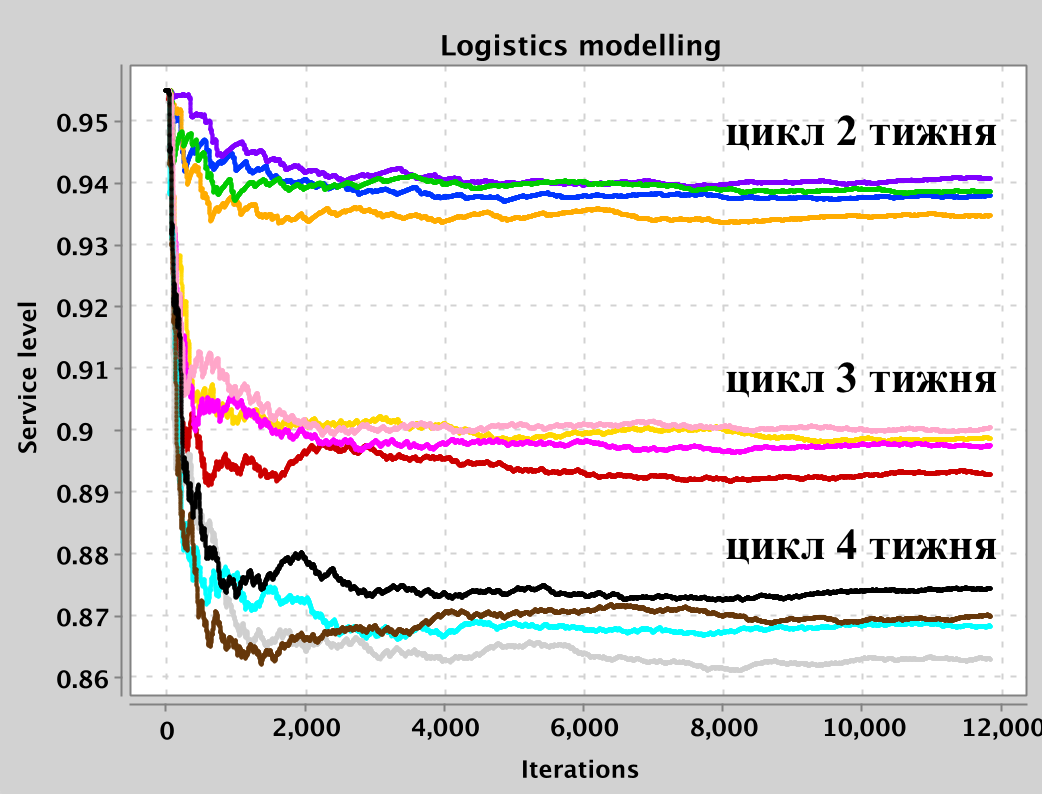
\includegraphics[width=0.6\textwidth]{graph_99}
	\caption{Динаміка зміни рівня сервісу для групи конфігурацій з базовим рівнем страхового запасу рівним $84.13$}
	\label{fig:graph_84}
\end{figure}

\begin{figure}[H]
	% \def\axisdefaultwidth{14cm}
	% \def\axisdefaultheight{10сm}
	\centering
	\begin{tikzpicture}
		\begin{axis}[
				legend style={font=\footnotesize,at={(1.6,1.0)},anchor=north east},
				xmin=0,
				xmax=10000,
				xlabel={Номер ітерації моделювання},
				xlabel style={yshift=-1cm},
				ylabel={Рівень сервісу},
				ylabel near ticks,
				ymajorgrids=true,
				grid style=dashed,
				line width=0.4mm,
				mark size=0pt,
				mark = none,
				smooth
			]
			\addplot table [x=i, y=1] {data/dynamic_97.csv};
			\addplot table [x=i, y=2] {data/dynamic_97.csv};
			\addplot table [x=i, y=3] {data/dynamic_97.csv};
			\addplot table [x=i, y=4] {data/dynamic_97.csv};
			\addplot table [x=i, y=5] {data/dynamic_97.csv};
			\addplot table [x=i, y=6] {data/dynamic_97.csv};
			\addplot table [x=i, y=7] {data/dynamic_97.csv};
			\addplot table [x=i, y=8] {data/dynamic_97.csv};
			\addplot table [x=i, y=9] {data/dynamic_97.csv};
			\addplot table [x=i, y=10] {data/dynamic_97.csv};
			\addplot table [x=i, y=11] {data/dynamic_97.csv};
			\addplot table [x=i, y=12] {data/dynamic_97.csv};
			\legend{5 складів; 2 тижня,6 складів; 2 тижня,7 складів; 2 тижня,8 складів; 2 тижня,5 складів; 3 тижня,6 складів; 3 тижня,7 складів; 3 тижня,8 складів; 3 тижня,5 складів; 4 тижня,6 складів; 4 тижня,7 складів; 4 тижня,8 складів; 4 тижня}
		\end{axis}
	\end{tikzpicture}
	% 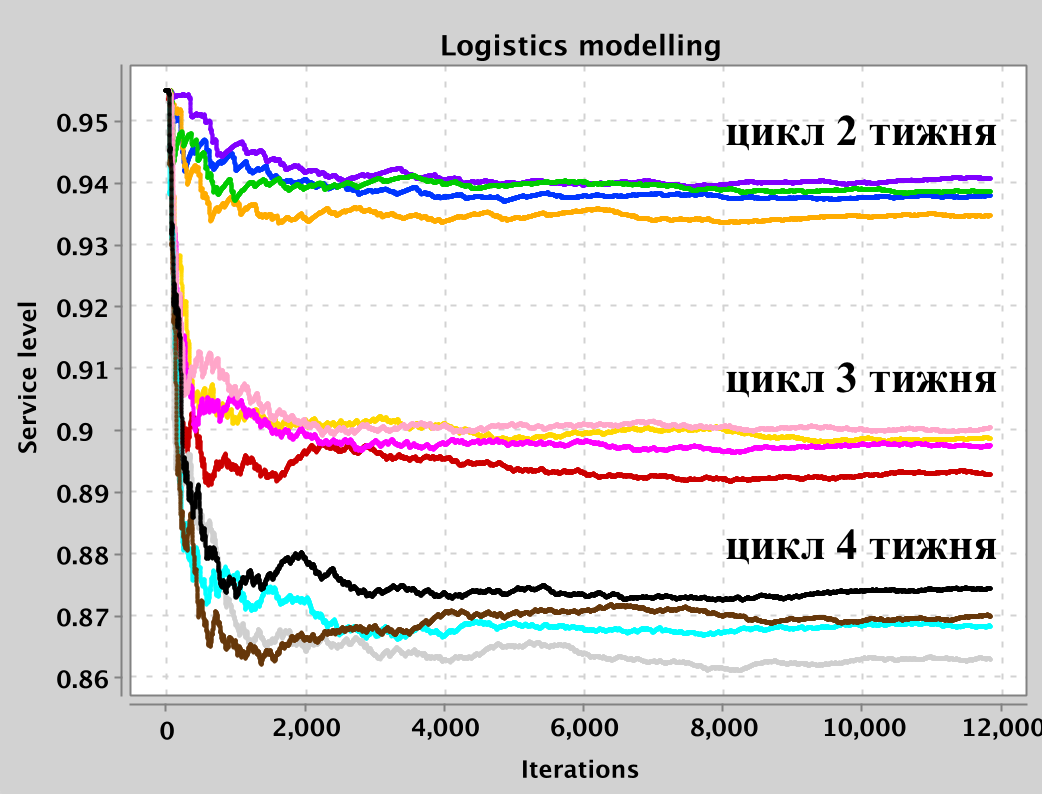
\includegraphics[width=0.6\textwidth]{graph_99}
	\caption{Динаміка зміни рівня сервісу для групи конфігурацій з базовим рівнем страхового запасу рівним $97.72$}
	\label{fig:graph_99}
\end{figure}

Наглядна графічна інтерпретація результатів з таблиці~\ref{tab:results} зображена на рисунку~\ref{fig:results}.

\begin{figure}[H]
	\centering
	\begin{tikzpicture}
		\begin{axis}[
				scaled y ticks = false,
				xlabel={Сумарні логістичні витрати},
				xlabel style={yshift=-1cm},
				ylabel={Мережевий рівень сервісу},
				ylabel near ticks,
				enlargelimits=false,
				line width=0.4mm,
				ymajorgrids=true,
				grid style=dashed,
			]
			\addplot+[
				only marks,
				scatter,
				mark=halfcircle*,
				mark size=2.9pt]
			table[meta=y]
				{data/results.csv};
		\end{axis}
	\end{tikzpicture}
	\caption{Результати експерименту моделювання конфігурацій логістичних систем}
	\label{fig:results}
\end{figure}

Проведемо аналіз отриманих результатів.
Незалежно від тривалості циклів замовлень рівень сервісу збільшується зі збільшенням кількості регіональних складів.
Це можна пояснити тим, що збільшується загальний розмір страхових запасів.
Мережевий рівень сервісу зменшується зі збільшенням тривалості циклів замовлень. Це пов'язано з тим, що при меншому циклі замовлень є більше можливостей на адаптацію до змін попиту.
Зі збільшенням базового рівня сервісу збільшується рівень мережевого сервісу.
Виходячи з проведеного аналізу, можна зробити висновок, що безліч ефективних рішень знаходиться в лівому верхньому кутку графіка (рис.~\ref{fig:results}). Залежно від пріоритету експерту по відношенню до критеріїв: сумарні логістичні витрати, мережевий рівень сервісу вибирається прийнятна конфігурація логістичної системи.

Подальше використання отриманих результатів пов'язане з визначенням стійкості рівня сервісу до різноманітних надзвичайних ситуацій. Отримані результати є основою для формування організаційної структури управління логістичною системою дистрибуції.


\section*{Висновки}
\addcontentsline{toc}{section}{Висновки}
Сучасні інструменти імітаційного моделювання дозволяють ефективно застосовувати його не тільки в наукових дослідженнях, а й як засоби для побудови систем підтримки прийняття рішень у бізнесі. 

Агентне моделювання дозволяє змоделювати систему максимально наближену до реальності, зробити значний крок у розумінні та управлінні сукупністю складних процесів.

Основним завданням даної практичної роботи була проектування, розробка та тестування мультиагентної системи для дослідження розподільчої логістичної системи.
Для досягнення поставленої мети роботи виконано наступні завдання:
\begin{enumerate}
    \item Розроблені вимоги до програмного забезпечення.
    \item Описана модель вхідних даних. 
    \item Спроектована архітектура програмного забезпечення. 
    \item Обґрунтувано вибір інструментальних засобів.
    \item Реалізована та протестована програмна система. 
    \item Проведено аналіз результатів дослідження. 
\end{enumerate}

\printbibliography[heading=bibintoc, title={Список джерел інформації}]


\end{document}
